\documentclass[t]{beamer}
%
% Choose how your presentation looks.
%
% For more themes, color themes and font themes, see:
% http://deic.uab.es/~iblanes/beamer_gallery/index_by_theme.html
%
\mode<presentation>
{
  \usetheme[compress]{Dresden}      % or try Darmstadt, Madrid, Warsaw, ...
  \usecolortheme{default} % or try albatross, beaver, crane, ...
  \usefonttheme{default}  % or try serif, structurebold, ...
  \setbeamertemplate{navigation symbols}{}
  \setbeamertemplate{caption}[numbered]
  \setbeamertemplate{footline}[frame number]
} 

\usepackage[english]{babel}
\usepackage[utf8x]{inputenc}
\usepackage{amsmath, amssymb}
\usepackage{graphicx}
\usepackage{comment} 
\usepackage{booktabs} %for tables
\usepackage{bm}
\usepackage{tabularx}
\usepackage{tabulary}
\usepackage{hyperref}
\usepackage{color, colortbl} %for row highlighting
\definecolor{LightCyan}{rgb}{0.88,1,1}
\usepackage[symbol*]{footmisc}
\hypersetup{
    colorlinks,
    citecolor=black,
    filecolor=black,
    linkcolor=black,
    urlcolor=black
    linktoc=all
}
\title[Mobile money risk sharing presentation]{Mobile Money and Risk Sharing Against Aggregate shocks}
\author[Emma Riley]{Emma Riley  \\
University of Oxford}
\institute[NOVAFRICA conference 2016l]{NOVAFRICA conference 2016}
\date{14th July 2016}

\begin{document}

\begin{frame}
  \titlepage
\end{frame}

\section{Introduction}

\subsection*{Outline}
\begin{frame}{Roadmap}
  \tableofcontents
\end{frame}

\subsection*{Motivation}
\begin{frame}[allowframebreaks]{Motivation}
\begin{itemize}
\item Households in developing countries are subject to a large amount of variability in income (Dercon and Krishnan, 1996), particularly those reliant on agriculture. 
\item Households
have developed informal risk sharing strategies to reduce the impact of shocks (Dercon, 2002).
\item Under perfect risk sharing within a village, households are able to insure themselves against idiosyncratic shocks but not aggregate shocks (Mace, 1991)
\item There is mixed evidence on whether perfect risk sharing occurs within the village (Townsend, 1994, de Weerdt \& Dercon, 2006, Udry, 1994 etc.)
\end{itemize}
\framebreak 

Mobile money services are a new tool allowing small amounts of money to cheaply, quickly and safely be sent around the country via a mobile phone. They can help households smooth consumption after an aggregate shock:
\begin{itemize}
\item Mobile money services can allow households to smooth aggregate shocks by giving them access to remittance networks of people outside their village to share risk with.  
\item If remittance receiving households share remittances with other households in the village then mobile money services might benefit the entire village. 
\end{itemize}
\end{frame}
\begin{frame}{Literature}
\begin{itemize}
\item Mobile money services have been shown to help the user smooth income shocks in Kenya (Jack \& Suri 2014) and to help households smooth their consumption after a natural disaster (Blumenstock et al 2015) 
\item Mbiti \& Weil (2011) find in Kenya that M-Pesa (the largest mobile money service in Kenya) changes the pattern of remittance by increasing the frequency and volume of urban-rural transfers. 
\item Yang \& Choi (2007) find that remittances allow households to smooth 60\% of a fall in consumption after a rainfall shock in the Philippines.
\end{itemize}
\end{frame}


\subsection*{This paper}
\begin{frame}{This paper}
I use panel data from Tanzania to
\begin{itemize}
\item confirm if households are able to smooth their consumption in response to idiosyncratic but not aggregate shocks
\item look at if the introduction of mobile money services allows users to smooth consumption after an aggregate (rainfall) shock
\item look at to what extent having mobile money users in a village also benefits non-users, allowing all households within the village to smooth their consumption after an aggregate shock. 
\end{itemize}
\end{frame}
\subsection*{Contribution}
\begin{frame}{Contribution to the literature}
\begin{itemize}
\item I add to the literature on whether idiosyncratic shocks are insured at the village level \pause
\item I separate out the impact of mobile money services on aggregate and idiosyncratic shocks, showing the benefit of mobile money is for aggregate shocks where risk sharing cannot take place within a village.  \pause
\item I compare self-reported droughts or floods to actual rainfall deviations  \pause	
\item I examine the extent that mobile money helps the entire village smooth consumption after an aggregate shock, not just the household receiving the remittance  \pause	
\item I provide evidence for a positive impact of mobile money services in Tanzania
\end{itemize}
\end{frame}
\begin{frame}{Findings}
\begin{enumerate}
\item I find that villages completely insure against idiosyncratic shocks but that in villages without mobile money services large rainfall shocks cause a 5\% reduction in consumption. \pause
\item I show that mobile money use provides insurance against aggregate shocks, resulting
in household consumption of users no longer being negatively impacted by an aggregate shock.\pause
\item I find a significant and positive effect of having more mobile money users in the village on
the consumption of everyone else in the village\pause
\item However non-mobile-money-users in villages with mobile money still experience a fall in consumption after an aggregate shock.
\end{enumerate}
\end{frame}


\section{Data}
\subsection*{Aggregate shock}
\begin{frame}[label=data]{Data}
My data comes from 3 waves of the Tanzanian National Panel survey from 2008-2013 covering 3,600 households in 409 enumeration areas in each wave \hyperlink{supplemental}{\beamerbutton{summary statistics}}.\\ \pause
Aggregate shocks:
\begin{enumerate}
\item dummy variable equal to one if the household reported a drought or flood in the year proceeding the survey wave. 13\% of households report a flood or drought per year.
\item dummy variable equal to one if rainfall in a year was more than 1 standard deviation in absolute value from the 40 year mean rainfall for that EA. 24\% of households experienced a 1 sd rainfall shock in a year. 

\end{enumerate}

\end{frame}

\subsection*{Mobile money statistics}
\begin{frame}{Mobile money use I}
Looking at mobile phone ownership: 
\begin{itemize}
\item 45\% of households owned
at least one mobile phone 2008-9, 
\item 62\% in 2010-11
\item 71\% in 2012-13. 
\end{itemize}
And mobile money services:
\begin{itemize}
\item introduced in 2009
\item 13\% of households
had used a mobile money service in 2010-11 
\item 38\% had by 2012-13.
\end{itemize}
\end{frame}
\begin{frame}{Mobile money use II}
\begin{figure}[label=MM chart]
\centering
\vspace{20pt}
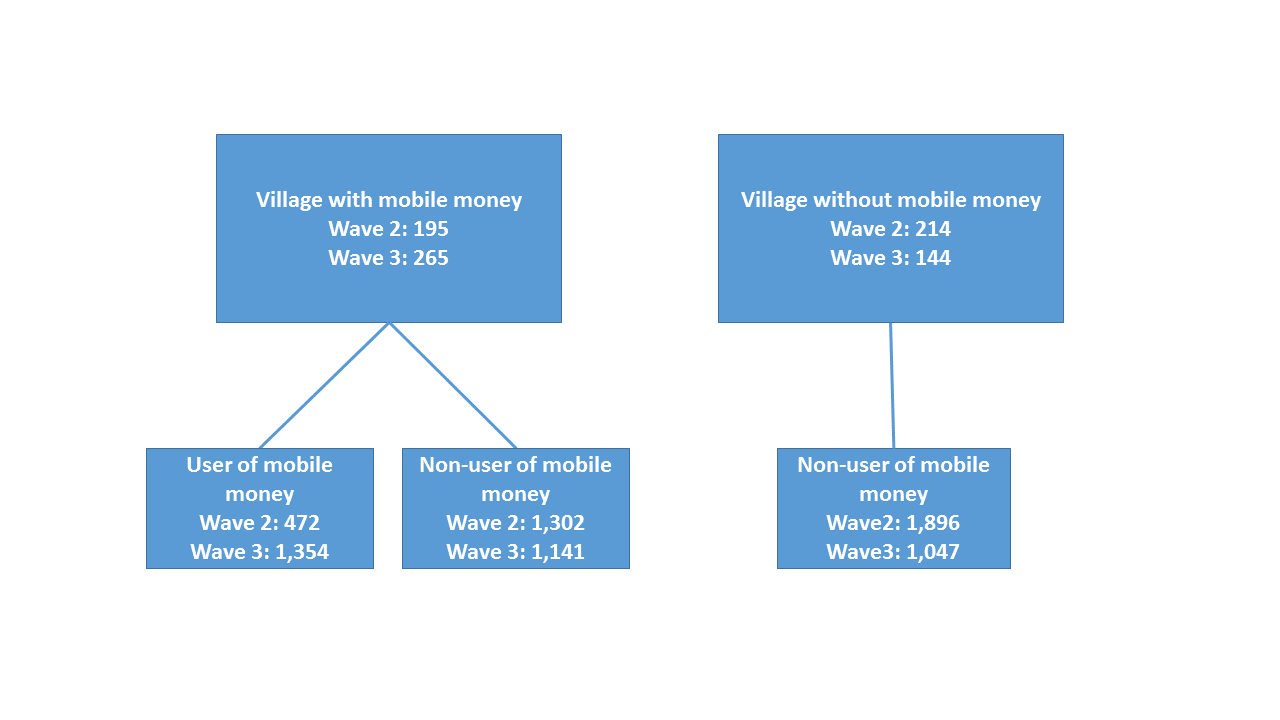
\includegraphics[width=\textwidth,trim= 0 3cm 0 3cm, clip=true, keepaspectratio]{users_chart_} 
\caption{Break down of villages and households by mobile money use} \label{fig:users chart}
\end{figure}
\end{frame}

\section{Estimation and identification Strategy}
\subsection*{Estimation Strategy}
\begin{frame}[allowframebreaks]{Estimation strategy}
I estimate the following panel difference-in-difference specification:
\begin{align} \label{eq: specification agg shock}
C_{jit} = &  \gamma_a AggShock_{jvt} + \mu MM_{jvt}   +\lambda VMM_{vt}  \notag \\
&  + \beta_m MM_{jvt}\cdot AggShock_{jvt} +\beta_v VMM_{vt}\cdot AggShock_{jvt} \notag \\
& + \bm{\theta X_{jvt}} +  \alpha_j + \delta_t + \varepsilon_{jvt} 
\end{align}
$C_{jvt}$ is household $j$'s per capita log consumption in village $v$ \\
$AggShock_{jvt}$ is a rainfall shock in village $v$ \\
$MM_{jvt}$ is mobile money use by individual $j$ \\
$VMM_{vt}$ is the proportion of mobile money users in the village \\
$\bm{X_{jvt}}$ is a vector of controls consisting of household demographics, financial service use and occupation dummies \\
$\alpha_j$ is a household fixed effect, $\delta_t$ is a time trend and $\varepsilon_{jvt}$ is a time varying error. 

\framebreak
This gives the following predictions for the empirical estimation:
\begin{description}
\item[Prediction 1] $\gamma_a<0$ so that rainfall shocks have negative effects on consumption.
\item [Prediction 2] For households in villages with at least one mobile money user, if remittances are perfectly shared within the village after an aggregate shock then  $\beta_v >0$ and $\beta_m=0$. 
\item [Prediction 3] If users of mobile money do not share remittances after an aggregate shock with other members of the village then $\beta_v=0$ and $\beta_m>0$.
\end{description}

\end{frame}
\subsection*{Identification}
\begin{frame}{Identification}
There are 2 self-selection effects which could bias my results
\begin{enumerate}
\item Selection by individuals into mobile money based on unobservable time-varying characteristics. This could bias $\mu$. \pause
\begin{itemize}
\item I am interested in the interaction of mobile money use with a random aggregate shock, $\beta_m$.	
\item I do not find that households which experience more rainfall shocks are more likely to use mobile money.\pause
\end{itemize}
\item Selection into EAs by agents based on unobservable time-varying village and household characteristics. \pause
\begin{itemize}
\item I check whether having a mobile money agent in the village is correlated with characteristics of the village and find no correlation. 
\item I perform a placebo test of future mobile money availability 
\end{itemize}
\end{enumerate}
 
\end{frame}
\section{Results and discussion}
\subsection*{Main results}
\begin{frame}[label=main results]{Main results}
\vspace{-10pt}
\begin{table}
  \centering
  \caption{Impact of rainfall shocks on consumption for mobile money users and non-users} \label{MM spill}
\resizebox{0.75\textwidth}{!}{\begin{tabular}{lcccccccc}
\multicolumn{7}{c}{Dependent variable: Log consumption per capita} \\\hline
& \multicolumn{3}{c}{ Self-reported shock} & \multicolumn{3}{c}{1 sd rainfall shock} \\ \cmidrule(r){2-4} \cmidrule(l){5-7}
 & (1) & (2) & (3)  & (4)  & (5) & (6) \\

  & Diff-in-diff & FE & FE & Diff-in-diff & FE &FE  \\ \hline
 &  &  &  & && \\
Rain shock & -0.049* & -0.046* & -0.005  & -0.042** & -0.044**  & 0.060   \\
 & (0.026) & (0.024) & (0.157) & (0.020) & (0.020) & 0.067 \\
Mobile money use & 0.137*** & -0.002 & -0.003 & 0.116*** & 0.004 & 0.004   \\
 & (0.023) & (0.023) & (0.023)  & (0.024) & (0.024) & (0.024) \\
\rowcolor{LightCyan}
Shock*MM use   & 0.037 & 0.107** & 0.083*  & 0.083** & 0.063*  & 0.076*  \\
   & (0.047) & (0.045) & (0.048) & (0.040) & (0.037) & (0.042) \\
Village MM use   & 0.095* & 0.094* & 0.098*  & 0.055 & 0.109* & 0.133**  \\
  & (0.052) & (0.056)  & 0.056) & (0.055) & (0.066) & (0.060)  \\
\rowcolor{LightCyan}
Shock*village MM use   & -0.071 & -0.104 & -0.213**  & 0.074 & 0.007 & -0.044 \\
& (0.096) & (0.081) & (0.096)   & (0.074) & (0.074) & (0.079)   \\

Observations & 9,281 & 9,281 & 9,281 & 9,281 & 9,281 & 9,281  \\
Number of households  &  & 3,807  & 3,807 &  & 3,807 & 3,807  \\
R-squared & 0.568 & 0.195 & 0.352 & 0.568 & 0.196 & 0.352  \\ 
Shock interactions & & & YES & & & YES \\
\hline
\end{tabular}}
 \end{table}
\end{frame}
\subsection*{Robustness}
\begin{frame}{Placebo test}
\vspace{-10pt}
\begin{table}
\centering
\caption{Placebo test of future mobile money use 2007-2009} \label{placebo}
\resizebox{0.85\textwidth}{!}{\begin{tabular}{lccccc} \multicolumn{5}{c}{Dependent variable: Log food consumption per capita} \\\hline
& \multicolumn{2}{c}{Placebo pre-mobile money data} & \multicolumn{2}{c}{Actual mobile money use data} \\ \cmidrule(r){2-3} \cmidrule(l){4-5}
 & (1) & (2) & (3) & (4) \\
 & Diff-in-diff & FE & Diff-in-diff  & FE \\ \hline
 &  &  &  &  &  \\
Rain shock &-0.05** & -0.04 & -0.07***  & -0.04 \\
 & (0.03) & (0.05) & (0.03)  & (0.04) \\
 \rowcolor{LightCyan} MM ever & -0.04 & -0.05 &    &  \\
 & (0.05) & (0.05) &  &  &  \\
MM use &  &  & 0.06** & 0.06** \\
 &  &  & (0.03) & (0.03) \\
 
\rowcolor{LightCyan} Rain shock*MM ever & 0.01 & 0.01 &  &  \\
 & (0.09) & (0.01) &  &  \\

Rain shock*MM use &  &  & 0.11**  & 0.12** \\
 &  &  & (0.05) & (0.06) \\
Observations & 2,332 & 2,332 & 9,567  & 9,567 \\
Number of households & 1,204 & 1,204 & 3,738 & 3,738 \\
R-squared & 0.369 & 0.225 & 0.276  & 0.101 \\
  \hline
\end{tabular}}
\end{table}
\end{frame}
\subsection*{Mechanism}
\begin{frame}{Floods or droughts}
\vspace{-10pt}
\begin{table}
\centering
\caption{Comparison of floods versus droughts} \label{flood drought}
\resizebox{0.68\textwidth}{!}{\begin{tabular}{lcccc} \multicolumn{5}{c}{Dependent variable: Log consumption per capita} \\\hline
& \multicolumn{2}{c}{Drought} & \multicolumn{2}{c}{Flood} \\ \cmidrule(r){2-3} \cmidrule(l){4-5}
 & (1) & (2) & (3) & (4)  \\
VARIABLES & Diff-in-diff & FE  & Diff-in-diff & FE \\ \hline
 &  &  &  &    \\
Shock & -0.06** & -0.05** & 0.02 & -0.01   \\
 & (0.02) & (0.02) & (0.03) & (0.03)  \\
Village MM use  & 0.09* & 0.10** & 0.07 & 0.11   \\
 & (0.05) & (0.05) & (0.05) & (0.06)   \\
Shock*village MM use & 0.16 & 0.02  & -0.03 & -0.06   \\
 & (0.16) & (0.17)  & (0.08) & (0.08)  \\
MM use  & 0.14*** & 0.01 & 0.112*** & 0.01 \\
 & (0.02) & (0.02) & (0.02) & (0.02) \\
Shock*MM use & 0.10* & 0.14* & 0.07 & 0.01  \\
 & (0.06) & (0.08)  & (0.04) & (0.05)  \\
Observations & 9,281 & 9,281  & 9,281 & 9,281\\
Number of households  & 3,807 & 3,807 & 3,807 & 3,807 \\
R-squared & 0.57 & 0.13  & 0.55 & 0.08  \\
 \hline
\end{tabular}}
\end{table}
\end{frame}
\begin{frame}{Robustness and mechanisms}
\begin{itemize}
\item Placebo test using 2007 data 
\item IV using distance travel time to the nearest mobile money agent
\item Propensity score matching on observable characteristics
\item Amount of remittances received after shocks
\item Impact of a mobile money agent on migration in and out of a village
\item Results by distance to the nearest agent
\item Urban-rural differences
\item Flood-drought differences
\item Test non-linearities in rainfall shocks
\item Exogeneity of rainfall shock
\item Other aggregate shocks
\end{itemize}
\end{frame}
\subsection*{Discussion}
\begin{frame}{Discussion}
Why is the consumption of non-mobile-money-users in villages with other mobile-money-users not smoothed after an aggregate shock? 
\begin{itemize}
\item Lack of information on who has received mobile money remittances and the extent that consumption of a household has fallen after an aggregate shock
\item Mobile-money-users are choosing to leave the village risk sharing arrangement and insure themselves against shocks within a wider network of family and friends 
\item Lack of norms for sharing after an aggregate shock
\item Breakdown of risk sharing after a large aggregate shock (Coate \& Ravallion, 1993)
\item Pressure from the remittance sender not to share
\end{itemize}
\end{frame}
\section{Conclusion}
\begin{frame}{Conclusion}
\begin{itemize}
\item I show that mobile money services help households smooth aggregate shocks which would otherwise lead to a 5\% fall in per capita consumption
\item This result holds primarily for droughts
\item I find that non-users in villages will mobile money still experience a drop in consumption after an aggregate shock
\item Future work should focus on how access to mobile money services is changing traditional geographically-based risk sharing networks
\end{itemize}
\end{frame}
\appendix

\begin{frame}[label=supplemental]
\begin{table}[htbp]

  \centering
  \caption{HH summary stats by wave} \label{HH sum}
    \resizebox{!}{0.4\textheight}{\begin{tabular}{lcccccc}
    \toprule
          & \multicolumn{2}{c}{Wave 1}        & \multicolumn{2}{c}{Wave 2} &      \multicolumn{2}{c}{Wave 3}   \\
    \midrule
          & Mean  & SD    & Mean  & SD    & Mean  & SD \\
    Per capita consumption &            743,386  &            725,334  &            862,266  &               782,264  &           1,011,279  &          1,090,465  \\
    Rural & 0.65  & 0.48  & 0.68  & 0.47  & 0.65  & 0.48 \\
    Rainfall shock & 0.18     & 0.38  & 0.09  & 0.29  & 0.20  & 0.40 \\
    Education of head (yrs) & 4.76  & 3.57  & 4.84  & 3.65  & 4.96  & 3.70 \\
    Age of head & 45.53 & 15.05 & 45.85 & 15.53 & 46.71 & 16.04 \\
    Head female & 0.25 & 0.43 & 0.26 & 0.43 & 0.28 & 0.446 \\
    Household size & 5.08  & 2.86  & 5.28  & 3.13  & 5.02  & 3.05 \\
    Mobile money use & 0.00  & 0.00  & 0.13  & 0.33  & 0.38  & 0.49 \\
    Own mobile & 0.45  & 0.50  & 0.62  & 0.48  & 0.71  & 0.45 \\
    Number of loans & 0.07  & 0.30  & 0.10  & 0.35  & 0.12  & 0.39 \\
    Bank account & .     & .     & 0.20  & 0.40  & 0.20  & 0.40 \\
    ROSCA & 0.04  & 0.20  & 0.05  & 0.22  & 0.04  & 0.19 \\
    Wealth index & -0.80 & 2.99 & 0.14 & 2.84 & -0.89 & 2.56 \\
        Agriculture/ Livestock & 0.60  & 0.49  & 0.56  & 0.50  & 0.55  & 0.50 \\
     Fishing & 0.02  & 0.14  & 0.01  & 0.12  & 0.01  & 0.12 \\
     Mining & 0.00  & 0.05  & 0.00  & 0.06  & 0.00  & 0.06 \\
     Tourism & 0.00  & 0.02  & 0.00  & 0.02  & 0.00  & 0.02 \\
     Employed: Government & 0.06  & 0.23  & 0.06  & 0.24  & 0.06  & 0.23 \\
     Parastatal & 0.01  & 0.08  & 0.01  & 0.08  & 0.01  & 0.07 \\
     Private sector & 0.09  & 0.28  & 0.11  & 0.31  & 0.12  & 0.33 \\
     NGO/religious & 0.01  & 0.09  & 0.01  & 0.08  & 0.01  & 0.09 \\
     Self-employed (non-agri) w employees & 0.02  & 0.16  & 0.03  & 0.18  & 0.03  & 0.16 \\
     Self-employed (non-agri) w/o employees & 0.15  & 0.35  & 0.14  & 0.35  & 0.15  & 0.36 \\
     Unpaid family work & 0.01  & 0.05  & 0.01  & 0.11  & 0.01  & 0.11 \\
          No job & 0.01  & 0.12  & 0.02  & 0.13  & 0.02  & 0.13 \\
    \bottomrule
    \end{tabular}}
    \end{table}
\hyperlink{data}{\beamerbutton{data}}
\end{frame}
\begin{frame}[label=idio]
\begin{table}[ht]
\centering
\caption{Household fixed effects regressions of different idiosyncratic shocks on consumption}
\resizebox{1.0\textwidth}{!}{\begin{tabular}{lccccc}
\multicolumn{6}{c}{Dependent variable: Log consumption per capita} \\\hline
 & (1) & (2) & (3) & (4) & (5)  \\
 & Household business failure & Loss of salaried employment & Chronic/ severe illness & Death of household member & Fire in home    \\ \hline
 &  &  &  & &   \\
 Shock & 0.077 & 0.014 & 0.036  & -0.010 & -0.017   \\
  & (0.065)  &  (0.099) & (0.067) & (0.040) & (0.078)  \\
Observations & 6,769 & 6,769 & 6,769 & 6,769 & 6,769 \\
Number of households  & 3,427 & 3,427 & 3,427 & 3,427 & 3,427 \\
 R-squared & 0.171 & 0.171 & 0.171 & 0.171 & 0.171 \\ \hline
\end{tabular}}
\end{table}
\hyperlink{main results}{\beamerbutton{results}}
\end{frame}
\end{document}